\documentclass{scrreprt}
\usepackage{etex}
\usepackage[ngerman]{babel}
\usepackage[utf8]{inputenc}
\usepackage[T1]{fontenc}
\usepackage{amsmath, amssymb}
\usepackage{graphicx}

\usepackage{pgfplots}
\pgfplotsset{compat=1.11}
\usepgfplotslibrary{external}
\usepackage{pgfplotstable}

\usepackage{booktabs}
\usepackage{multirow}
\usepackage{longtable}
%\usepackage{ulsy}
%\usepackage{pst-all}
\usepackage{picture}
\usepackage[automark]{scrpage2}
\usepackage{caption}
\pagestyle{scrheadings}
\ihead[]{Friedrich Hübner 2897111}
\ohead[]{Fiona Paulus 2909625} 

\author{Friedrich Hübner 2897111\\
Fiona Paulus 2909625}
\title{Computerphysik\\Hausarbeit 4}

\begin{document}
\maketitle
\newpage

\chapter*{Der Differentialgleichungssolver}
Für den DGL-Solver wird das Runge-Kutta-Verfahren mit den Fehlbergkoeffizienten und automatischer Schrittweitensteuerung aus der Vorlesung verwendet. Die Berechnung aller Werte erfolgt genau nach diesem Verfahren.

\section*{Programm (abgabe4\_runge\_kutta.cpp)}
In dieser Datei befindet sich der DGL-Solver, der von allen anderen Programmen eingebunden wird.\\

Mit der Funktion 'runge\_kutta\_init(f, $t_0$, $y_0$)' wird der DGL-Solver initialisiert. Dabei ist $f: \mathbb{R} \times \mathbb{R}^n \to \mathbb{R}^n$ die Differentialgleichung ($y' = f(t,y)$), $t_0 \in \mathbb{R}$ der Anfangszeitpunkt und $y_0 \in \mathbb{R}^n$ der Anfangswert.\\

Mit der Funktion 'runge\_kutta\_iterate()' wird ein Schritt ausgeführt und die neue optimale Schrittweite berechnet.\\

Außerdem werden in der Datei Operatoren für Vektorarithmetik (+,+=,-,*) und für Ausgabe von Vektoren (<\.<) überladen. Zusätzlich gibt es noch Funktionen für den Betrag von Vektoren und das Skalar- und Kreuzprodukt.  

\chapter*{Aufgabe 3}
\section*{Allgmeine Hinweise}
Das Programm wurde unter Windows 10 mit "g++ -o abgabe4\_3.exe -Wall -Wextra -std=c++0x -O2 -static abgabe4\_3.cpp"\;kompiliert.

\section*{a)}
Die Bewegungsgleichung lautet einfach:
\begin{align}
m\ddot{\vec{x}} &= e\dot{\vec{x}} \times \vec{B}\\
				&= e\dot{\vec{x}} \times \left(\cfrac{\mu_0}{4\pi}\cfrac{3\vec{x}(\vec{x} \cdot \vec{m}) - \vec{m}\cdot\vec{r}^2}{|r|^5}\right)  
\end{align}

Der Dipol wurde Richtung z-Achse gelegt: $\vec{m} = (0,0,m)^T$.\\

Für $\vec{y} = (\vec{x},\dot{\vec{x}})$ gilt nun:\\
\begin{align}
\dot{\vec{y}} = \left(\dot{\vec{x}},  \cfrac{e}{m}\dot{\vec{x}} \times \left(\cfrac{\mu_0}{4\pi}\cfrac{3\vec{x}(\vec{x} \cdot \vec{m}) - \vec{m}\cdot\vec{r}^2}{|r|^5}\right)\right)  
\end{align}

\section*{b) Programm (abgabe4\_3.cpp)}
Das Programm benutzt den Fehlberg-DGL-Solver. Die verwendete Funktion f ist dabei in a) gegeben. Die Anfangsbedingungen muss man in das Programm eintragen. Das Programm simuliert 100s und gibt aller 0.1s Simulationzeit die aktuelle Zeit, Position und Geschwindigkeit aus.  

\section*{c)}
Da der Dipol in z-Richtung angeordnet ist, sind die Feldlinien am Äquator parallel zur z-Achse. Also startet das Proton mit $\vec{v} = (-1000,0,v_z)^T$.
\subsection*{1. $\mathbf{v_z = 100km/s}$}
\subsubsection*{i)}
\begin{center}
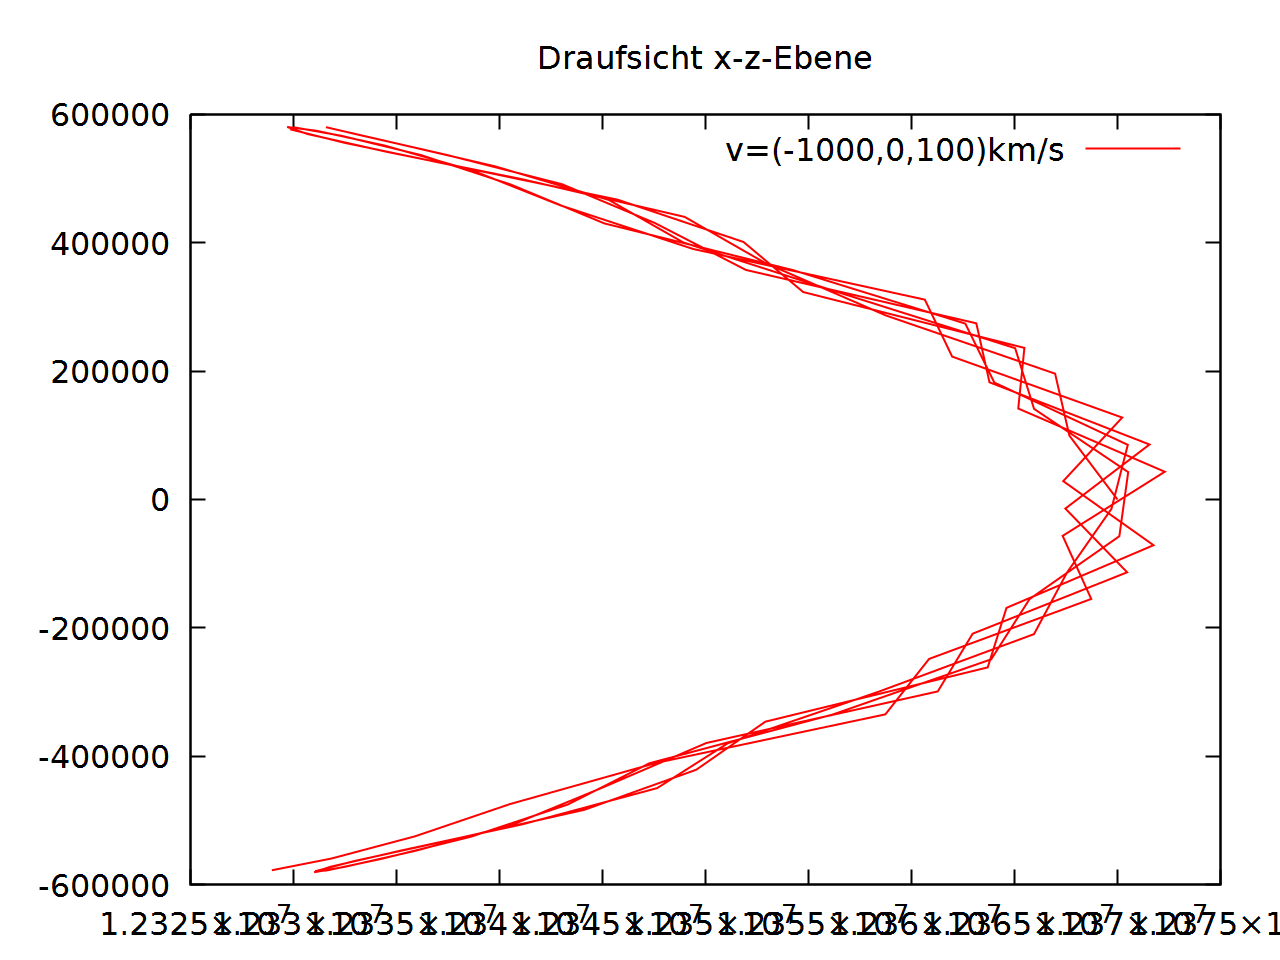
\includegraphics[scale=0.25]{plot_1_i.png}
\end{center}
\subsubsection*{ii)}
\begin{center}
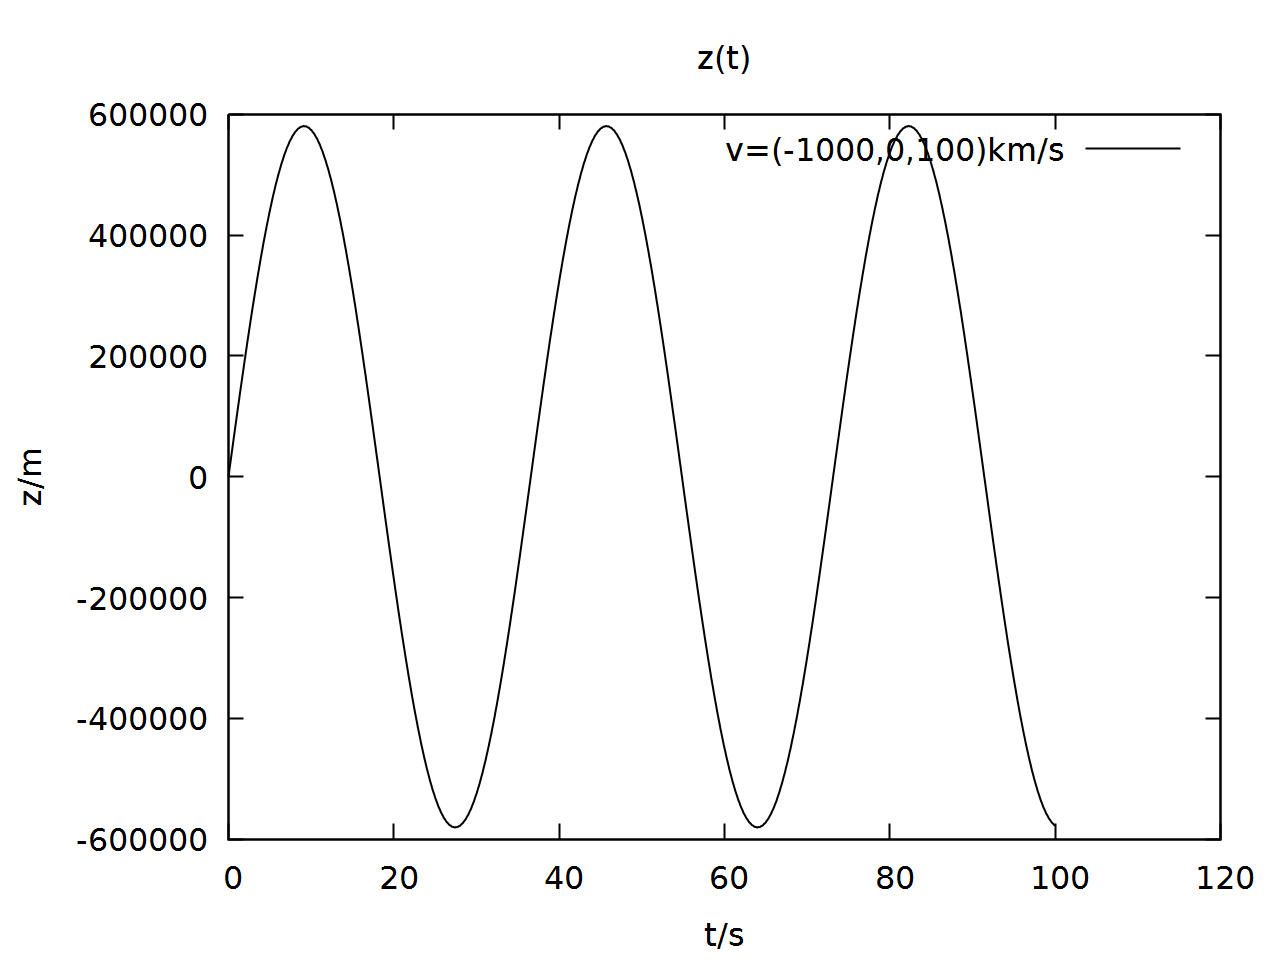
\includegraphics[scale=0.25]{plot_1_ii.png}
\end{center}
\subsubsection*{iii)}
\begin{center}
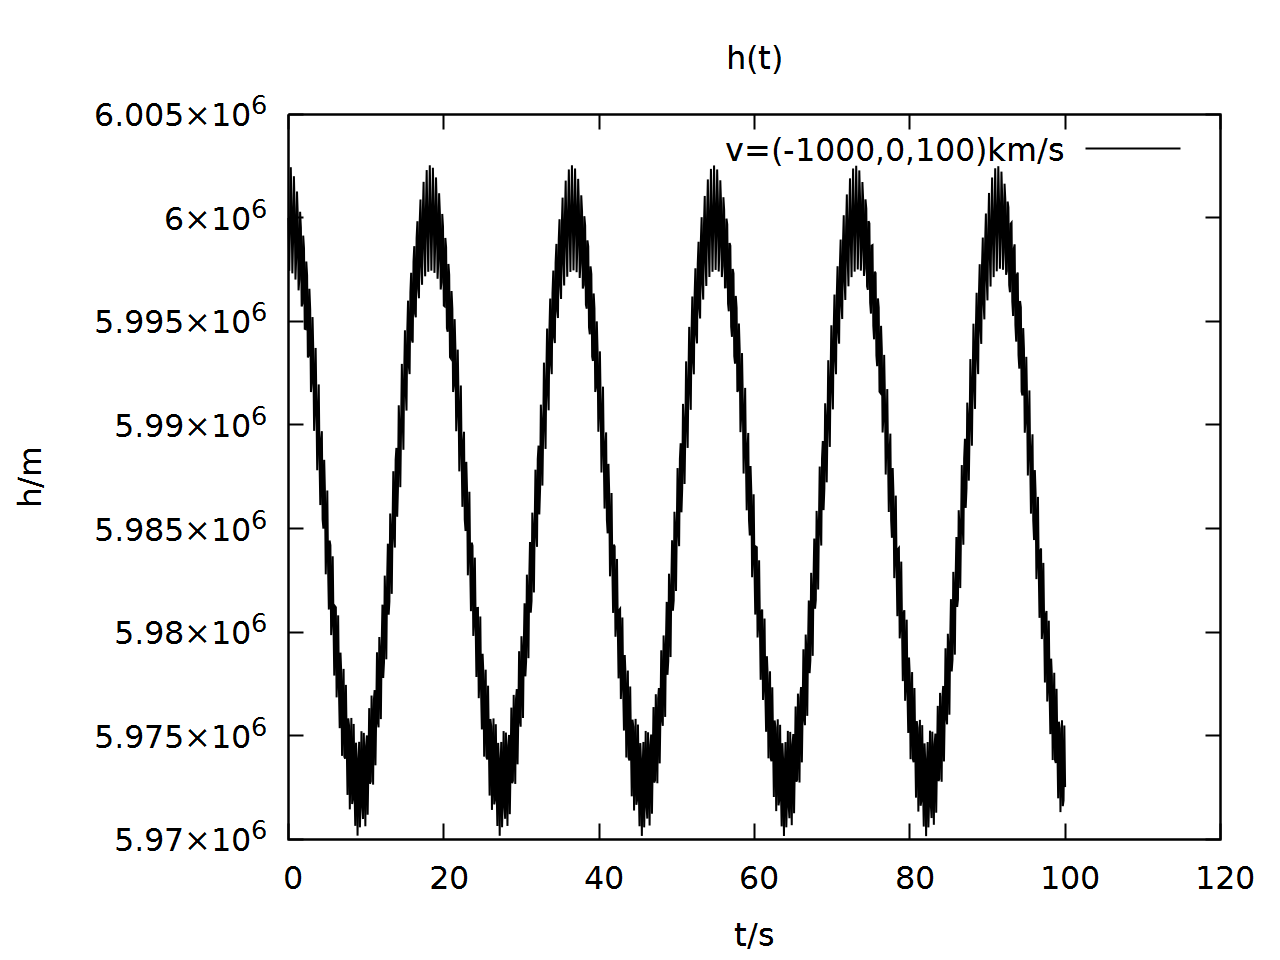
\includegraphics[scale=0.25]{plot_1_iii.png}
\end{center}

\subsection*{2. $\mathbf{v_z = 1000km/s}$}
\subsubsection*{i)}
\begin{center}
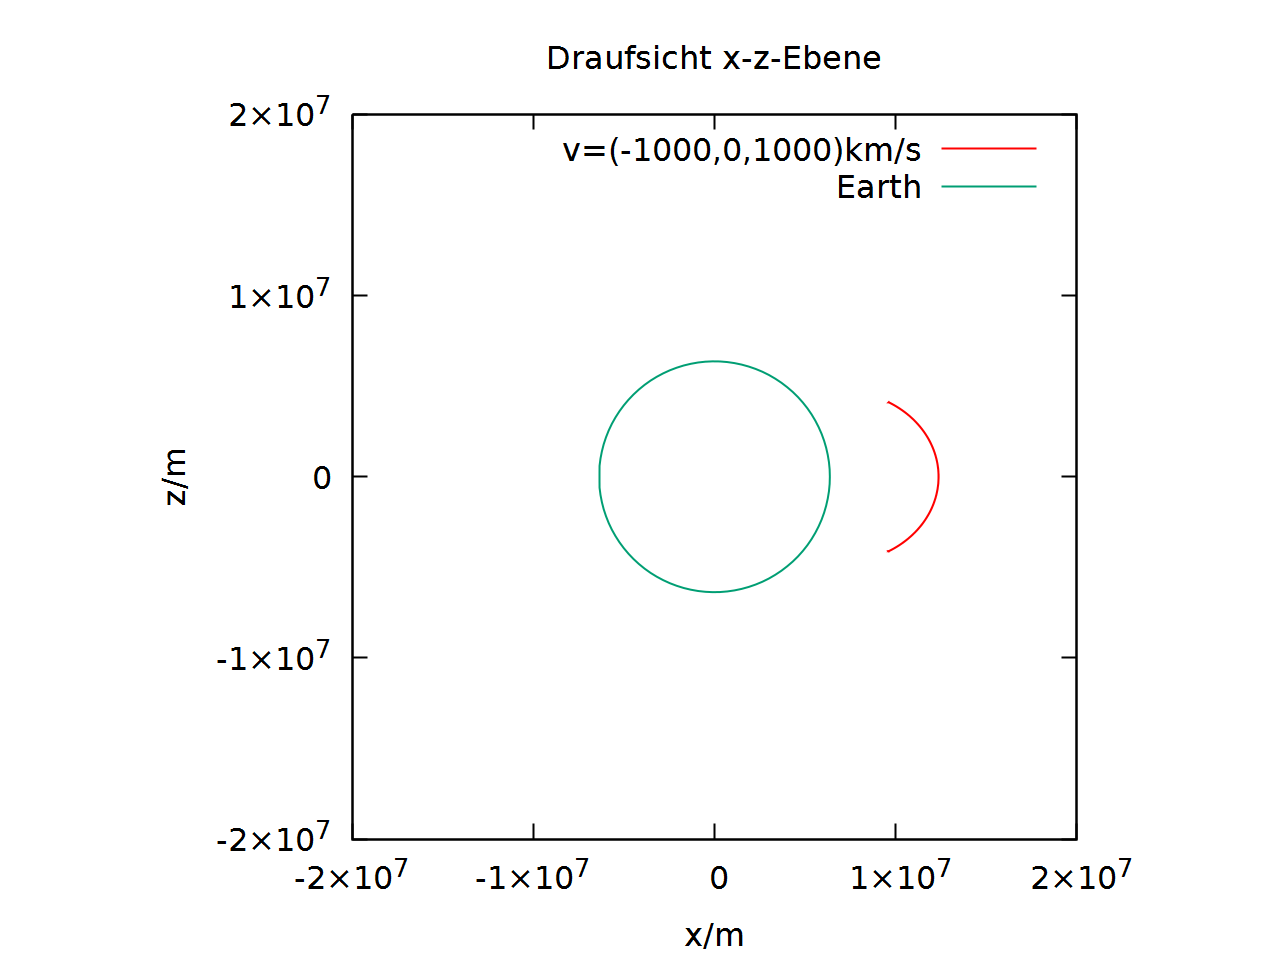
\includegraphics[scale=0.25]{plot_2_i.png}
\end{center}
\subsubsection*{ii)}
\begin{center}
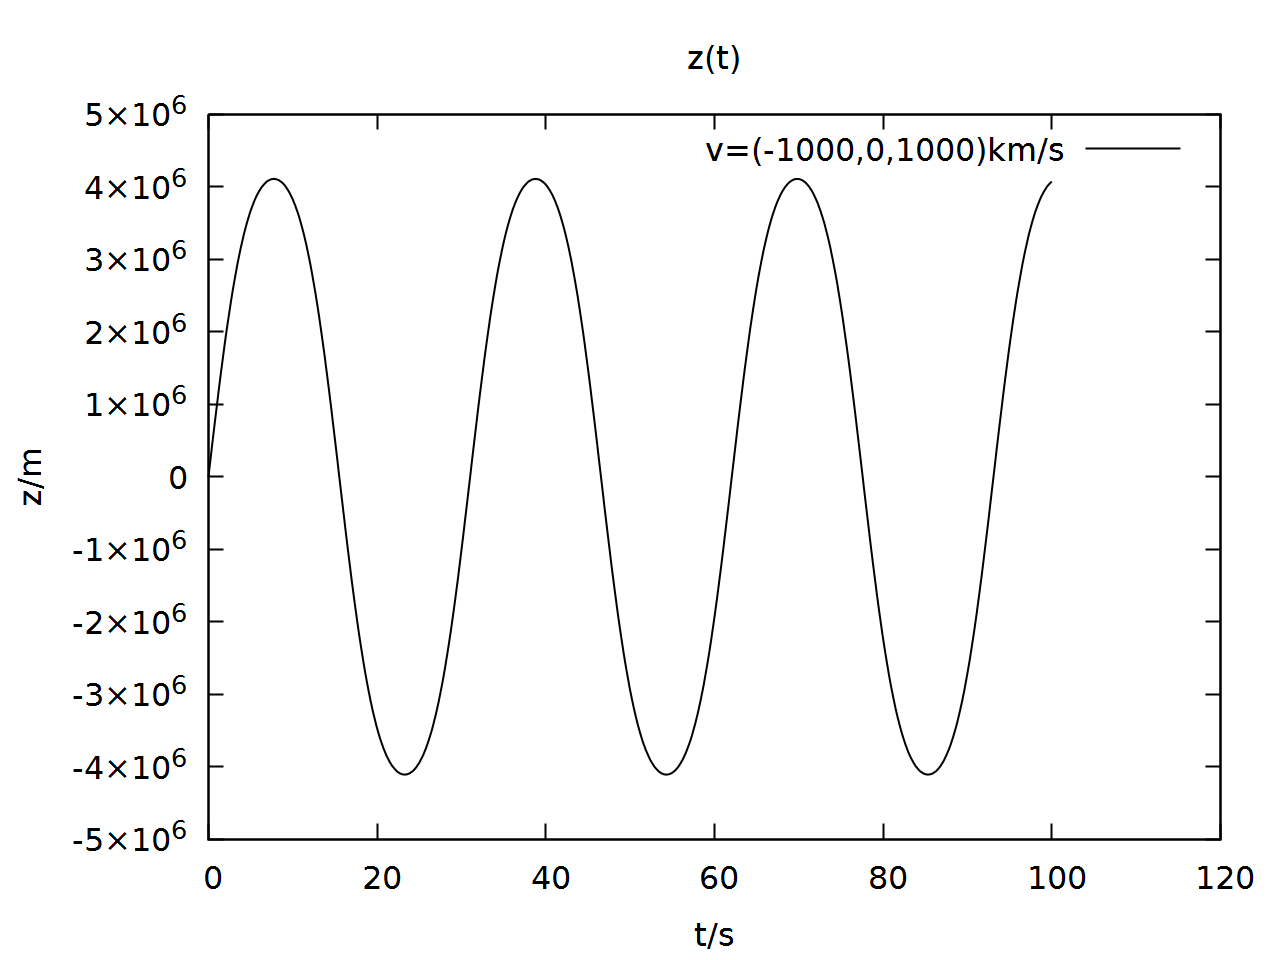
\includegraphics[scale=0.25]{plot_2_ii.png}
\end{center}
\subsubsection*{iii)}
\begin{center}
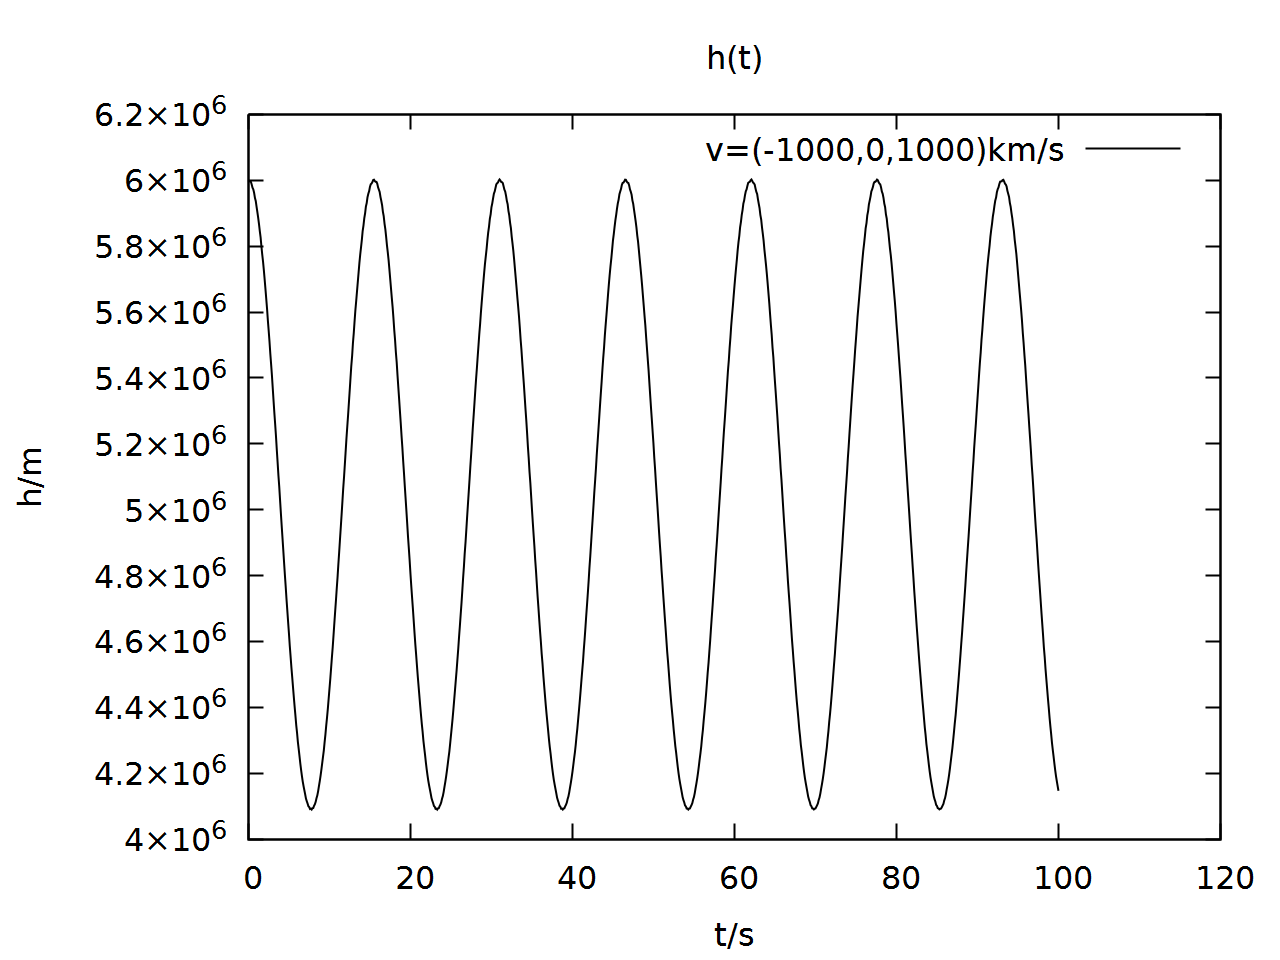
\includegraphics[scale=0.25]{plot_2_iii.png}
\end{center}

\subsection*{3. $\mathbf{v_z = 3000km/s}$}
\subsubsection*{i)}
\begin{center}
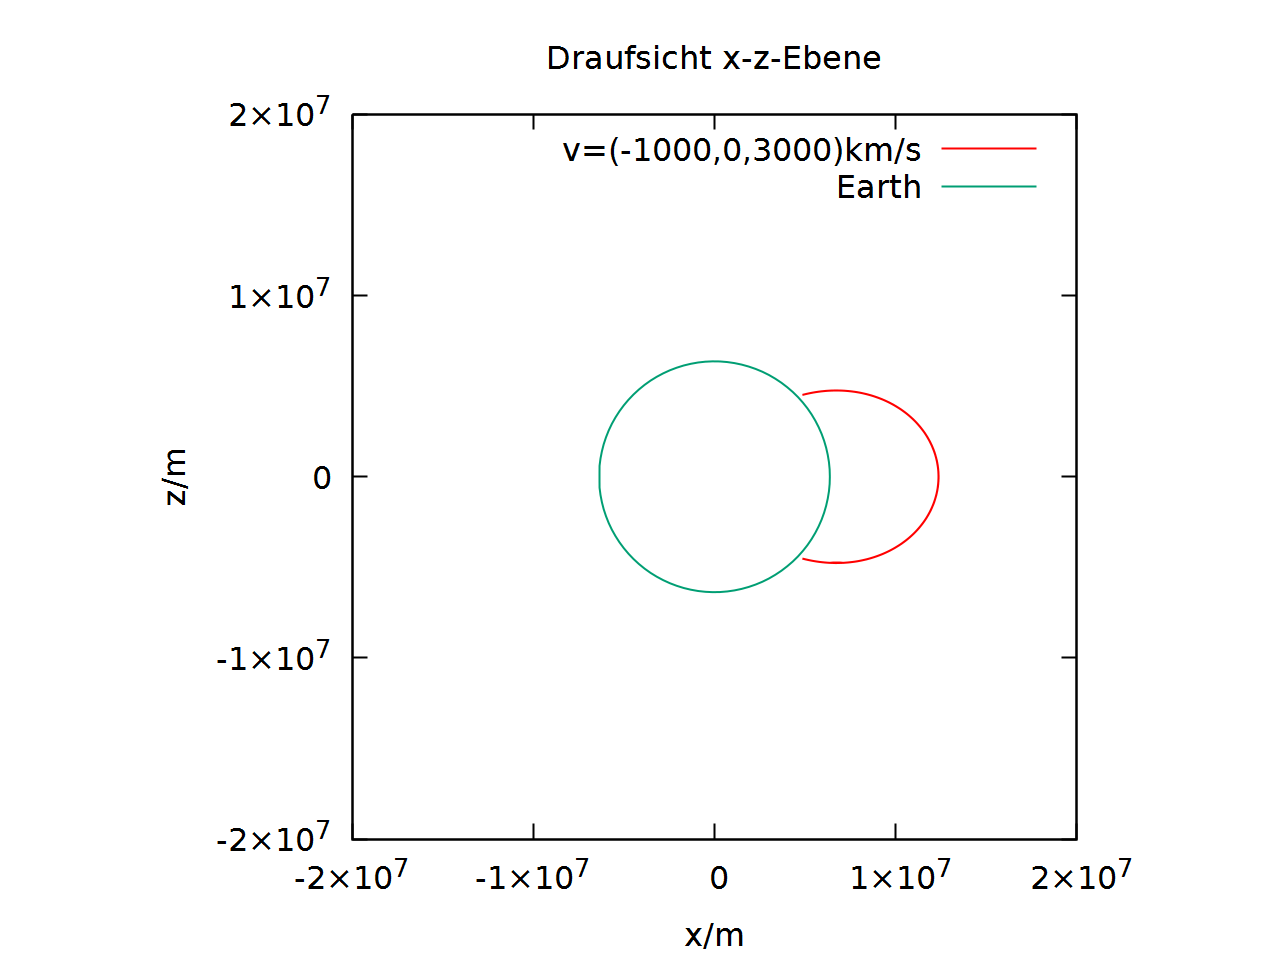
\includegraphics[scale=0.25]{plot_3_i.png}
\end{center}
\subsubsection*{ii)}
\begin{center}
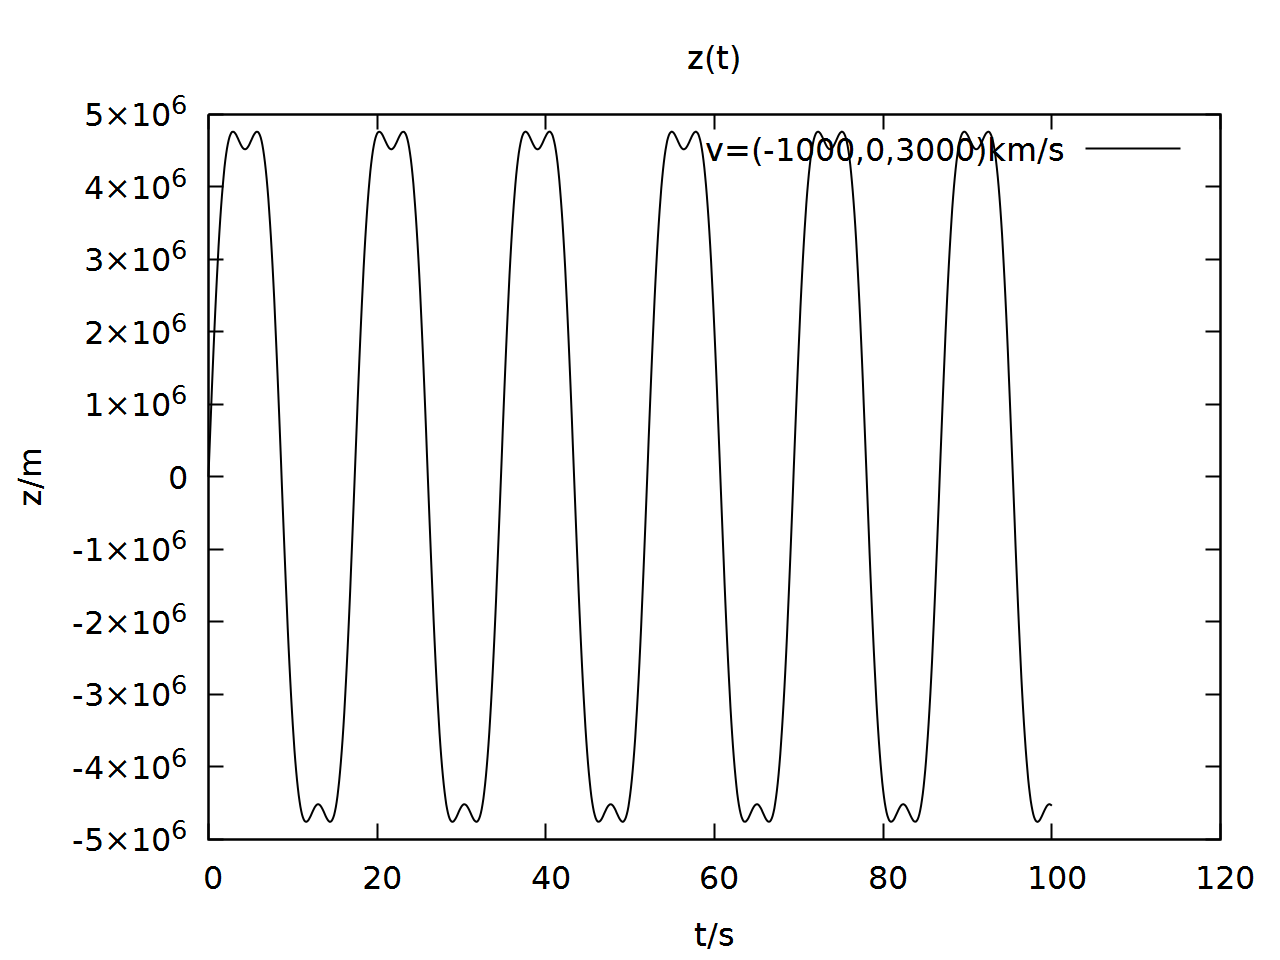
\includegraphics[scale=0.25]{plot_3_ii.png}
\end{center}
\subsubsection*{iii)}
\begin{center}
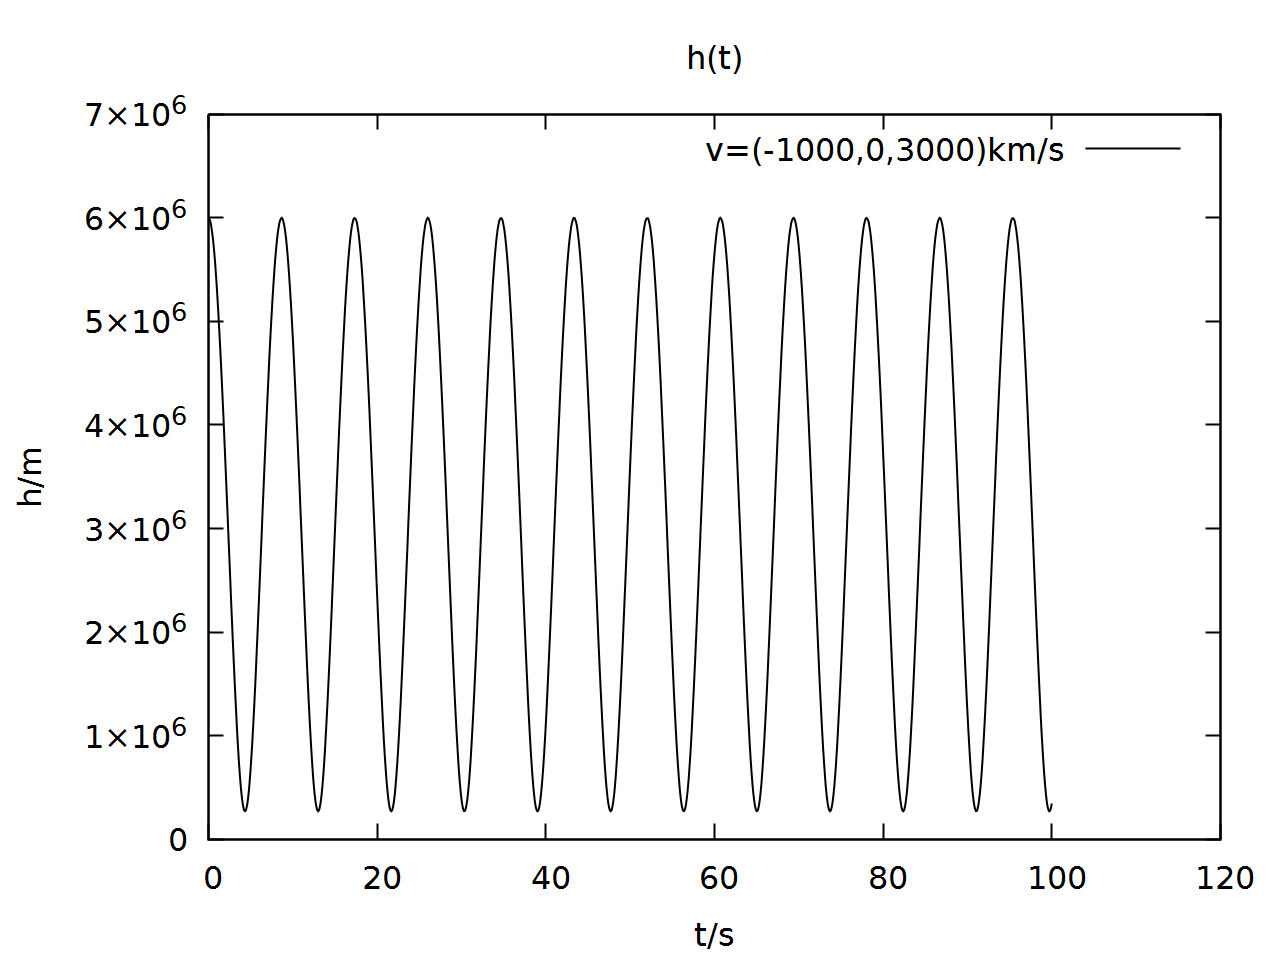
\includegraphics[scale=0.25]{plot_3_iii.png}
\end{center}



\section*{Sonstige abgegebene Dateien}
\subsection*{plot\_i.plt, plot\_ii.plt, plot\_iii.plt}
Die Plot-Dateien für die Diagramme für jeweils Fall i), ii), iii)
\subsection*{1.txt, 2.txt, 3.txt}
Die Ausgabedateien für die einzelnen Anfangswerte
\end{document}